\section{Naming\-Base Class Reference}
\label{classNamingBase}\index{NamingBase@{NamingBase}}
Inheritance diagram for Naming\-Base::\begin{figure}[H]
\begin{center}
\leavevmode
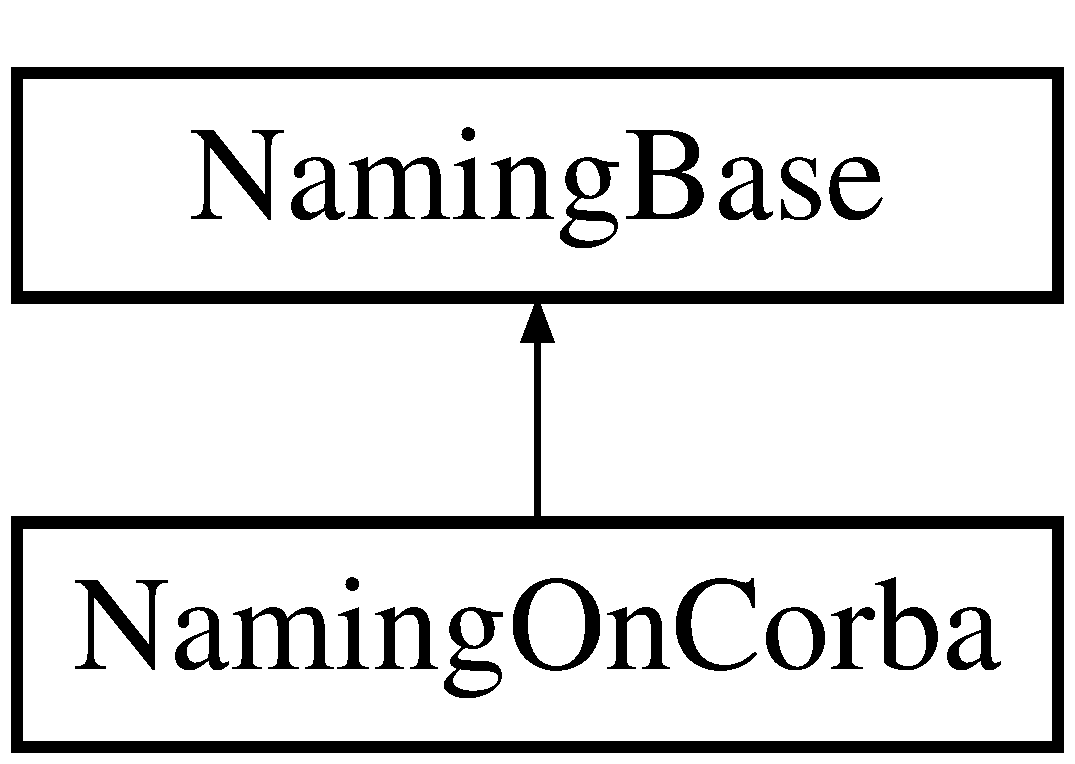
\includegraphics[height=2cm]{classNamingBase}
\end{center}
\end{figure}
\subsection*{Public Member Functions}
\begin{CompactItemize}
\item 
{\bf \_\-\_\-del\_\-\_\-} ()
\item 
{\bf bind\-Object} (name, rtobj)
\item 
{\bf unbind\-Object} (name)
\end{CompactItemize}


\subsection{Member Function Documentation}
\index{NamingBase@{Naming\-Base}!__del__@{\_\-\_\-del\_\-\_\-}}
\index{__del__@{\_\-\_\-del\_\-\_\-}!NamingBase@{Naming\-Base}}
\subsubsection{\setlength{\rightskip}{0pt plus 5cm}Naming\-Base::\_\-\_\-del\_\-\_\- ()}\label{classNamingBase_NamingBasea0}




Reimplemented in {\bf Naming\-On\-Corba} {\rm (p.\,\pageref{classNamingOnCorba_NamingOnCorbaa0})}.\index{NamingBase@{Naming\-Base}!bindObject@{bindObject}}
\index{bindObject@{bindObject}!NamingBase@{Naming\-Base}}
\subsubsection{\setlength{\rightskip}{0pt plus 5cm}Naming\-Base::bind\-Object (name, rtobj)}\label{classNamingBase_NamingBasea1}




Reimplemented in {\bf Naming\-On\-Corba} {\rm (p.\,\pageref{classNamingOnCorba_NamingOnCorbaa1})}.\index{NamingBase@{Naming\-Base}!unbindObject@{unbindObject}}
\index{unbindObject@{unbindObject}!NamingBase@{Naming\-Base}}
\subsubsection{\setlength{\rightskip}{0pt plus 5cm}Naming\-Base::unbind\-Object (name)}\label{classNamingBase_NamingBasea2}




Reimplemented in {\bf Naming\-On\-Corba} {\rm (p.\,\pageref{classNamingOnCorba_NamingOnCorbaa2})}.

The documentation for this class was generated from the following file:\begin{CompactItemize}
\item 
{\bf Naming\-Manager.py}\end{CompactItemize}
